\documentclass{article}
\usepackage[utf8]{inputenc}
\usepackage{hyperref}
\usepackage{float}
\usepackage{graphicx}
\graphicspath{{./images/}}

\title{Super Mario World AI}
\author{Siebren Cosijn}
\begin{document}
    \maketitle

    \section{Introduction}
    \begin{figure}[H]
    \centering
    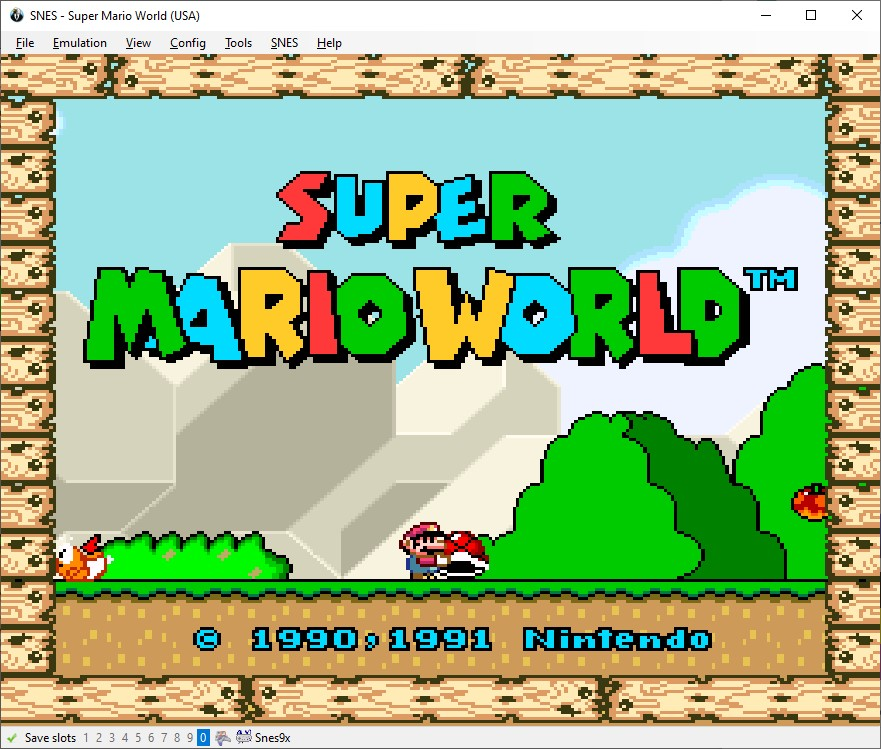
\includegraphics[width=.85\textwidth]{start-screen}
    \end{figure}
    \begin{itemize}
        \item Reinforcement learning
        \item OpenAI Gym\footnote{\url{https://github.com/openai/gym}} - RL library
        \item Gym Retro\footnote{\url{https://github.com/openai/retro/}} - Game integration for gym
    \end{itemize}

    \section{Goals}
    Learn to complete level(s) of the game Super Mario World

    \section{Preprocessing}
    \subsection{Discrete Actions}
    \begin{itemize}
        \item x and y same function
        \item movement: none, left, right, down, up
        \item jump: none, spin, jump
        \item special: none, special
        \item $5*3*2=30$ discrete actions
    \end{itemize}
    \begin{figure}[H]
    \centering
    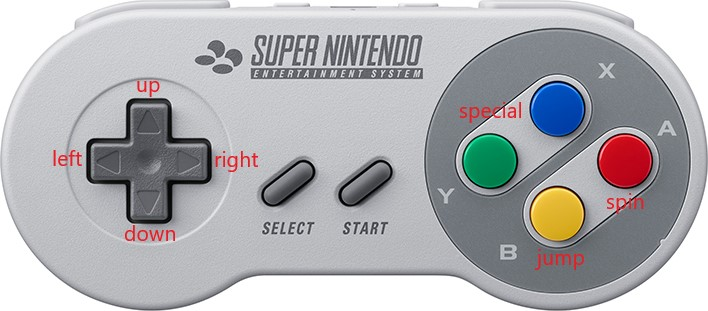
\includegraphics[width=.85\textwidth]{snes-controller-annot}
    \end{figure}
    \subsection{Frame Manipulation}
    \subsubsection*{Skip frames}
    \begin{itemize}
        \item Very little change from frame to frame (x FPS)
        \item Consider every 4th frame
        \item Reduced training time
    \end{itemize}
    \subsubsection*{Stack frames}
    \begin{itemize}
        \item Use 4 subsequent observations for training
        \item Direction of movement
    \end{itemize}
    \subsubsection*{Resize frames}
    \begin{itemize}
        \item 84x84
        \item Grayscale
        \item Reduced memory requirement
    \end{itemize}
    \begin{figure}[H]
        \centering
        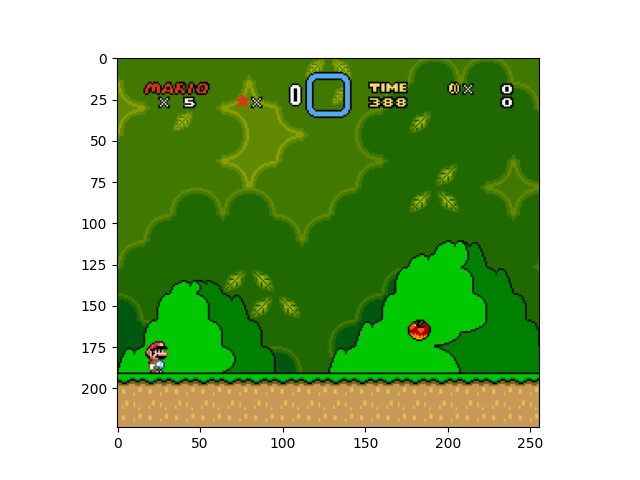
\includegraphics[height=5cm]{original}\hfill
        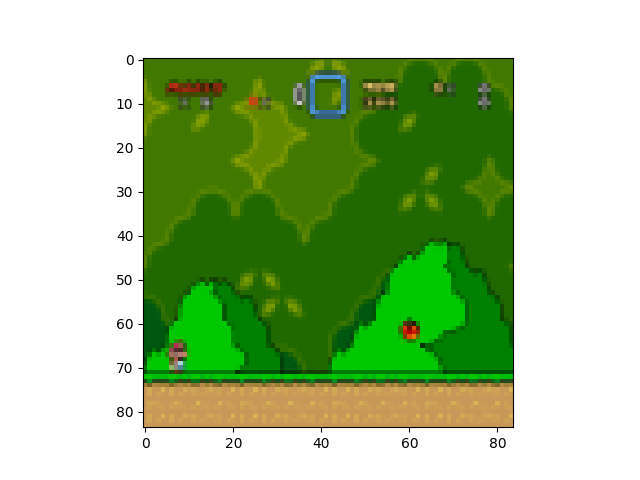
\includegraphics[height=5cm]{scaled}
    \end{figure}

    \section{Model}
    \subsection{Algorithm}
    \begin{itemize}
        \item Proximal Policy Optimization (PPO)
        \item Policy based algorithm
        \item Stable Baselines library\footnote{\url{https://github.com/DLR-RM/stable-baselines3}}
    \end{itemize}
    \subsection{Reward}
    \subsubsection*{Positive reward}
    \begin{itemize}
        \item move right $\Rightarrow$ small positive reward
        \item reach checkpoint/end of level $\Rightarrow$ large positive reward
    \end{itemize}
    \subsubsection*{Negative reward}
    \begin{itemize}
        \item move left $\Rightarrow$ small penalty
        \item lose life $\Rightarrow$ large penalty
    \end{itemize}

    \section{Training}
    Sample initial states by taking random number of no-ops on reset.
    No-op is assumed to be action 0.

    Make end-of-life == end-of-episode, but only reset on true game over.
    Done by DeepMind for the DQN and co. since it helps value estimation.

    \section{Results}
\end{document}